\documentclass[12pt, a4paper, openright]{book}


\usepackage{amsmath}
\usepackage{graphicx}
\usepackage{listings}
\usepackage{float}
\usepackage{enumitem}
\usepackage{setspace}
\usepackage{datetime}
\usepackage{parskip}
\usepackage{hyperref}  % for citing URLs

\lstset{breaklines=true}
\pagestyle{plain}
\newcommand{\HRule}{\rule{\linewidth}{0.5mm}}
\newdateformat{mydate}{\monthname[\THEMONTH] \THEYEAR}

\hoffset        -1in
\voffset        -1in
\topmargin      15mm
\headheight     3mm
\headsep        12mm
\oddsidemargin  30mm    
\evensidemargin 20mm
\textheight     245mm
\textwidth      160mm
\footskip       13mm

%added on may 29 2014
%\linespread{1.3}
\onehalfspacing
%added on may 29 2014

\begin{document}

\frontmatter
\begin{titlepage}
\begin{center}
\begin{spacing}{1.0}

% Upper part of the page. The '~' is needed because \\
% only works if a paragraph has started.

% Title
~\\[0.3cm]
{ \LARGE \bfseries  Experimental implementation of a cognitive Base 
Transceiver Station in GSM band using OpenBTS and spectrum sensing 
techniques\\[1.2cm] }

\textbf{\large Dual Degree Dissertation}\\[1.2cm]

{Submitted in partial fulfilment of the requirements for the degree 
of\\[0.1cm]
Master of Technology\\[0.3cm]
by\\[0.3cm]}

{\LARGE Swrangsar Basumatary \\[0.1cm]}
{09d07040 \\[1.1cm]}
{Supervisor \\[0.1cm]}
{\LARGE Prof.~S~N~Merchant \\[1.3cm]}


\includegraphics[width=0.21\textheight]{iitbLogo}~\\[0.9cm]
Department of Electrical Engineering\\[0.2cm]
\textbf{\large IIT Bombay}\\[1.3cm]


\vfill

% Bottom of the page
{\large \today}

\end{spacing}
\end{center}
\end{titlepage}

\chapter*{\centering{Declaration of Academic Ethics}}

I declare that this written submission represents my ideas in my own words
and where others' ideas or words have been included, I have adequately cited
and referenced the original sources. I also declare that I have adhered to all
principles of academic honesty and integrity and have not misrepresented or
fabricated or falsified any idea/data/fact/source in my submission. I
understand that any violation of the above will be cause for disciplinary
action by the Institute and can also evoke penal action from the sources which
have thus not been properly cited or from whom proper permission has not been
taken when needed.

\vspace{1.5cm}

\begin{tabular}{lll}
\rule{40mm}{0pt}        & \rule{50mm}{0pt}       & \rule{60mm}{0pt} \\
Date:\dotfill           &                        & \dotfill \\
                        &                        & Swrangsar Basumatary \\
                        &                        & (Roll 09d07040)\\
\end{tabular}

\chapter*{\centering{Abstract}}
The explosive proliferation of mobile phones and other wireless communication
devices has rendered the spectrum an insufficient resource. To make things
worse, there exists a widespread underutilization of the spectrum. \gls{cr}
offers to tackle this problem by finding the unused frequency bands
in the spectrum (also known as spectrum holes) and allocating them to the
secondary users (SUs) for use. Hence, CR makes the usage of spectrum more
efficient.

We demonstrate the capabilities of \gls{cr} by developing a 2-frequency CR Test-Bed
and a 4-frequency CR Test-Bed. Primary users (PUs) and SUs are made to
coexist in the same frequency band. Energy detection method is used for the
spectrum sensing. PUs switch from their frequency band of operation to an
unused frequency band as soon as the activity of PUs is detected.
\chapter*{\centering{Acknowledgement}}
I would like to express my sincere gratitude to \textbf{Prof~S~N~Merchant}
for giving me the opportunity to work in this project and also for his
invaluable guidance and encouragement during the course of the project. I am
grateful to Prof~V~M~Gadre for his valuable feedback and suggestions. I thank
Prof~V~Rajbabu for always reminding us to be serious in our project work.

I am indebted to my project partner Abrar Ahmad 
for all the help in practically carrying out this work. I appreciate the 
support rendered to me by SPANN lab and its members like Chaitanya Pande, 
Sudipto Mondal, Kartik Sudarshan, Sagar Sharma, Joy Khan and so on. Finally,
I would like to thank my friends for their constant support and
encouragement.

\vspace{1.5cm}

\begin{flushright}
\textbf{Swrangsar Basumatary} \\
IIT Bombay
\end{flushright}

\setcounter{tocdepth}{2}
\tableofcontents

\listoffigures
%\setlength{\parindent}{0pt}
%\setlength{\parskip}{1em}
\setlength\arraycolsep{2pt}

\mainmatter
\chapter{Introduction}
\section{Background}
The electromagnetic radio spectrum is a natural resource that remains 
underutilized \cite{haykin05}.
It is licensed by governments for use by transmitters and receivers.
With the explosive proliferation of cell phones and other wireless 
communication devices,
we cannot afford to be lavish in using our spectral resources anymore.

In November 2002, the Spectrum Policy Task Force, a group under the Federal
Communications Commission(FCC) in the United States, published a report saying
\cite{repFCC}, 
\begin{quote}
``In many bands, spectrum access is a more significant problem than physical 
scarcity of spectrum, in large part due to legacy command-and-control 
regulation that limits the ability of potential spectrum users to obtain such 
access.''
\end{quote}

If we were to scan the radio spectrum even in metropolitan places where it's
heavily used, 
we would find that \cite{staple04}:
\begin{enumerate}
	\item some frequency bands are unoccupied most of the time,
	\item some are only partially occupied and
	\item the rest are heavily used.
\end{enumerate}

\begin{figure}
\centering
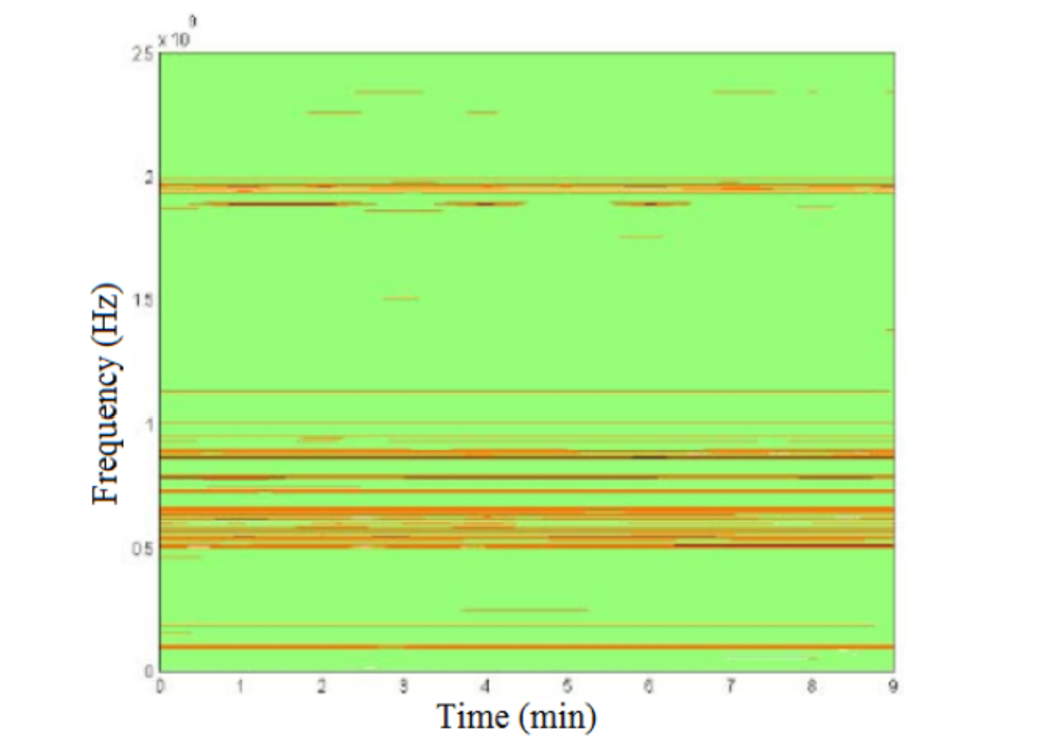
\includegraphics[width=0.7\textwidth]{../images/freqUsage}
\caption{Frequency usage of the Spectrum}
\label{freqUsage}
\end{figure}

The underutilization of spectral resources leads us to think in terms of 
\emph{spectrum holes}, which are defined as \cite{kolodzy01}:
\begin{quote}
\emph{A spectrum hole is a band of frequencies assigned to a primary user, 
but, at a particular time and specific geographic location, the band is not 
being utilized by that user.
}
\end{quote}

The spectrum can be better utilized by enabling secondary users (users who are
not licensed to use the services) to access spectrum holes unoccupied by 
primary users at the location and the time in question. 
\emph{Cognitive Radio}, which includes software-defined radio, has been 
promoted as the means to make efficient use of the spectrum by exploiting the 
existence of spectrum holes \cite{haykin05}\cite{mitola99}\cite{mitola00}.

\section{Cognitive Radio}
One of the definitions of Cognitive Radio is \cite{haykin05}:
\begin{quote}
\emph{Cognitive radio is an intelligent wireless communication system that is
aware of its surrounding environment (i.e., outside world), and uses the 
methodology of understanding-by-building to learn from the environment and 
adapt its internal states to statistical variations in the incoming RF stimuli
by making corresponding changes in certain operating parameters (e.g., 
transmit-power, carrier-frequency, and modulation strategy) in real-time, with
two primary objectives in mind:
\begin{itemize}
	\item highly reliable communications whenever and wherever needed;
	\item efficient utilization of the radio spectrum.
\end{itemize}}
\end{quote}

Besides, a cognitive radio is also reconfigurable. This property of cognitive 
radio is provided by a platform known as \emph{software-defined radio}. 
Software-defined Radio (SDR) is basically a combination of two key 
technologies: digital radio, and computer software.

\section{Contribution of this Thesis}

A cognitive base transceiver station is developed to demonstrate the efficient 
utilization of spectrum by allowing secondary users to make use of the 
frequency bands that are already licensed to primary users but that are not 
being used at that particular time and space.

\begin{enumerate}
    \item A 2-frequency system is developed where as soon as the presence of 
    primary users is detected in $F_1$  the secondary BTS switches from $F_1$ 
    to $F_2$ and vice-versa.
    \item The 2-frequency system is extended to a 4-frequency one where
    two of the four frequency channels always remain occupied. The secondary
    system switches to one of the two unused frequency channels.
    \item For sensing the frequency channels the energy detection based
    spectrum sensing method has been used and for peak detection the method 
    called CUSUM has been used. The frequency used by the secondary users is
    sensed continuously and as soon as the presence of primary users in that 
    frequency is detected the secondary finds an underutilized frequency 
    nearby and switches to that frequency.  
\end{enumerate}



\section{Organization of this Thesis}
The remaining chapters of this document are organized as follows. Chapter 2 
briefly touches upon the GSM system architecture and the GSM protocol 
architecture. Chapter 3 introduces Software Defined Radio (SDR) and some of the
tools that make SDR possible like the Universal Software Radio Peripheral 
(USRP N210) and the GNU Radio software package. Various parts of the OpenBTS 
software are described in Chapter 4. Chapter 5 reviews various techniques of 
spectrum sensing and gives a comparison among them. Chapter 6 describes the 
Cognitive Radio (CR) Test-Bed that we developed using OpenBTS. Flowgraphs of
the algorithms developed while making the CR Test-Bed are also given in
Chapter 6. Finally, Chapter 7 concludes this document.

\chapter{GSM}

\section{Overview}

GSM (Global System for Mobile Communications, originally Groupe Sp\'ecial Mobile), is a very popular standard that describes protocols for second generation (2G) digital cellular networks used by mobile phones. GSM networks usually operate in the 900 MHz, 1800 MHz or 1900 MHz bands. It supports a full data rate of 9.6 kbits/sec or 14.4 kbits/sec using better codecs.


\section{System Architecture}

A GSM Public Land Mobile Network (PLMN) consists of at least one Service Area managed by a Mobile Switching Center (MSC) connected to the Public Switched Telephone Network  (PSTN).

\begin{figure}
\centering
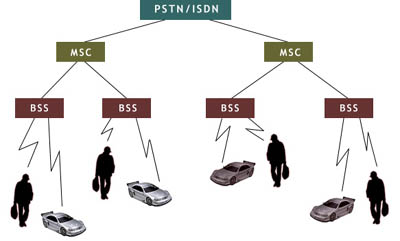
\includegraphics[scale=0.7]{archPLMN}
\caption[GSM PLMN architecture]{The architecture of a GSM Public Land Mobile Network (PLMN).
\emph{Source: \url{http://wireless.arcada.fi/MOBWI/material/CN\_1\_2.html}}}
\end{figure}

The network structure can be divided into the following discrete sections:
\begin{itemize}
\item Base Station Subsystem
\item Network and Switching Subsystem
\item Operation Subsystem
\end{itemize}


\subsection{Base Station Subsystem (BSS)}

A base station subsystem consists of
\begin{itemize} 
\item a Base Station Controller (BSC) and
\item at least one Base Transceiver Station (BTS) for Mobile Stations (MS). A mobile station can be a cell phone, or any electronic equipment such as a Personal Digital Assistant (PDA) with a phone interface.
\end{itemize}

The area served by a single BTS is considered a Network Cell. One or more BTSs are managed by a single BSC.  A group of BSSs can be managed as a Location Area (Location Area) provided all those BSSs are being managed by the same MSC.


\begin{figure}
\centering
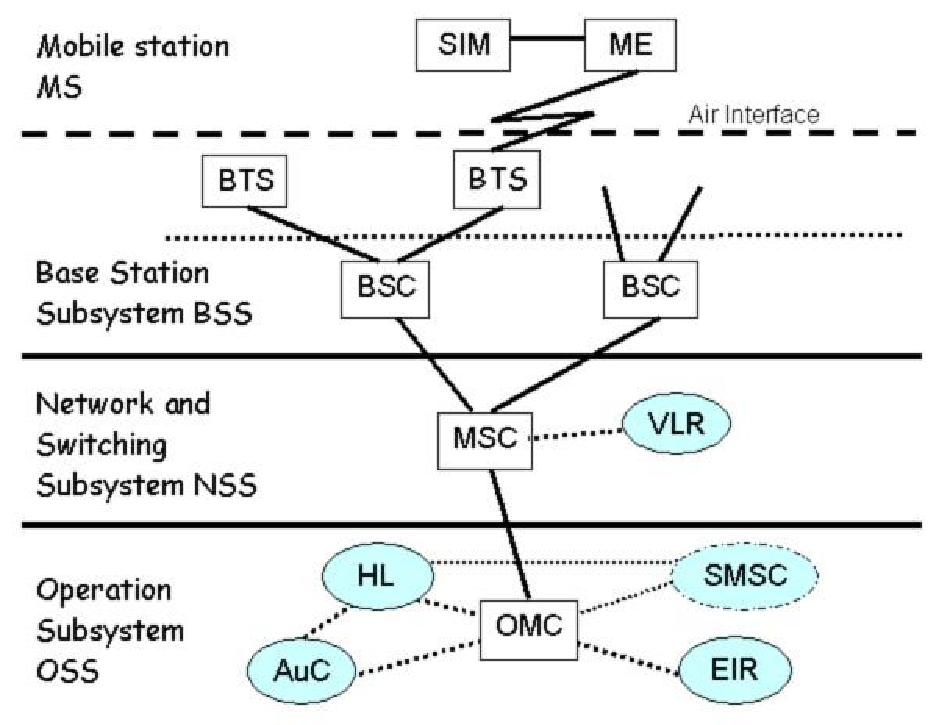
\includegraphics[scale=0.7]{archMSCServiceArea}
\caption[Network architecture for a single MSC Service Area]{The GSM network architecture for a single MSC controlled Service Area.
\emph{Source: \url{http://wireless.arcada.fi/MOBWI/material/CN\_1\_2.html}}}
\end{figure}


An MSC may also be connected via a Gateway MSC (GMSC) to other MSCs or the Public Switched Telephone Network (PSTN) with the Integrated Services Digital Network (ISDN) option. The Inter-Working Function (IWF) of a GMSC makes it possible to connect the circuit switched data paths of a GSM network with the PSTN/ISDN.

\begin{figure}
\centering
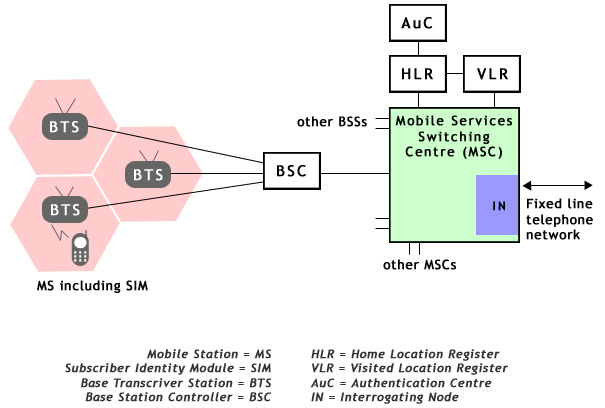
\includegraphics[scale=0.7]{gsmNetworkComponents}
\caption[GSM network components]{GSM network components.
\emph{Source: \url{http://wireless.arcada.fi/MOBWI/material/CN\_1\_2.html}}}
\end{figure}




\subsection{Network and Switching Subsystem (NSS)}

The NSS is made up of an MSC and a Visitor Location Register (VLR). An MSC 
\begin{itemize} 
\item sets up, controls and shuts down connections
\item handles call charges
\item manages additionals services like call forwarding, call blocking, etc.
\end{itemize}

A VLR contains all the subscriber data of the phones being served by the accompanying MSC. It contains their location data too. The VLR also maintains data about the SIMs that do not belong to the network but have roamed into the network. The area served by an MSC is called a MSC/VLR service area.

\begin{figure}
\centering
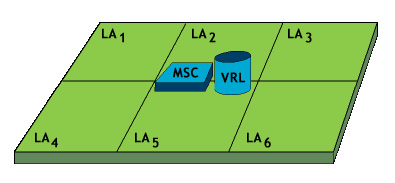
\includegraphics[scale=0.7]{mscvlrServiceArea}
\caption[MSC/VLR Service Area]{MSC/VLR Service Area.
\emph{Source: \url{http://wireless.arcada.fi/MOBWI/material/CN\_1\_2.html}}}
\end{figure}

\subsection{The Operation Subsystem (OSS)}

The OSS consists of :
\begin{itemize}
\item the Operation and Maintenance Center (OMC)
\item the Authentication Center (AuC)
\item the Home Location Register (HLR)
\item the Equipment Identity Register (EIR)
\end{itemize}

The OSS is responsible for
\begin{itemize}
\item network management functions like service provisioning, network configuration, fault management, etc.
\item billing calls
\item administering subscribers
\end{itemize}

The AuC controls all the encryption algorithms used for verifying the SIMs. The EIR contains the serial numbers of all the MSs (mobile phones) being served. The HLR contains the subscriber data and location data of all the SIMs in different parts of the network.

\subsection{GSM Network Areas}

The area covered by a GSM operator is called a PLMN Service Area. A PLMN service area is made up of several MSC/VLR service areas. The hierarchy of service areas is as follows:
\begin{itemize}
\item PLMN service area,
\item MSC/VLR service area,
\item Location Area and
\item Network Cell
\end{itemize}
\begin{figure}
\centering
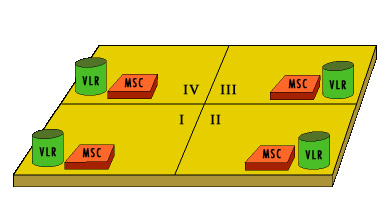
\includegraphics[scale=0.7]{PLMNServiceArea}
\caption[A PLMN Service Area for a GSM operator]{A PLMN Service Area for a GSM operator.
\emph{Source: \url{http://wireless.arcada.fi/MOBWI/material/CN\_1\_2.html}}}
\end{figure}



\section{Protocol Architecture}
The data communication protocols in a GSM network are implemented to work over the bearer\footnote{A bearer data channel is a channel that carries call content i.e.
one that does not carry signaling.} data channel. 
The GSM protocol architecture is structured into three independent planes:
\begin{itemize}
 \item user plane
 \item control plane
 \item management plane
\end{itemize}
\begin{figure}
\centering
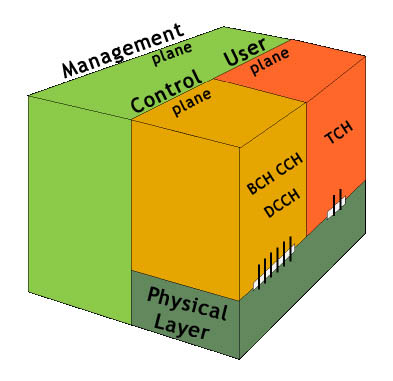
\includegraphics[scale=0.7]{gsmPlanes}
\caption[GSM protocol architecture planes]{GSM protocol architecture planes.
\emph{Source: \url{http://wireless.arcada.fi/MOBWI/material/CN\_1\_3.html}}}
\end{figure}

The user plane defines protocols for handling the voice and user data. 
At the Um interface, the traffic control channel (TCH) is used to carry the user data.


The control plane defines protocols for controlling connections by using signalling data.
The signalling data are carried over logical channels called Dm-channels (wireless analog of the D-channels for wired interface).
The spare capacities of the Dm-channels are used for carrying user data.
Eventually all logical channels have to multiplexed onto the physical channel.


The management plane takes care of the coordination between different planes.
It also manages functions related to the control and/or user planes.
The management plane handles things like network configuration, network fault, etc.

\begin{figure}
\centering
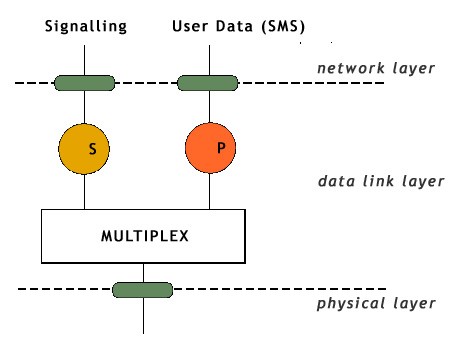
\includegraphics[scale=0.7]{logicalChannelsUserControl}
\caption[Logical channels for user plane data and control plane signalling]{Logical channels for user plane data and control plane signalling.
\emph{Source: \url{http://wireless.arcada.fi/MOBWI/material/CN\_1\_3.html}}}
\end{figure}

\subsection{Signalling Transmission}
In GSM, the network nodes exchange signaling information with each other to establish, control and terminate connections.
The various interfaces in a GSM network are:
\begin{itemize}
 \item MS-BTS: Um
 \item BTS-BSC: Abis
 \item BSC-MSC: A
 \item MSC-VLR: B
 \item MSC-HLR: C
 \item VLR-HLR: D
 \item MSC-MSC: E
 \item MSC-EIR: F
 \item VLR-VLR: G
\end{itemize}

The Um interface is the only interface that uses the wireless physical medium for carrying signals. The rest of the interfaces all use wired and digital mediums.

\subsubsection{\uppercase{Data Link Layer (Layer 2) protocols}}

\begin{description}
 \item [Link Access Protocol, Dm-channel (LAPDm)] is a layer 2 protocol that provides safe, reliable connections to layer 3 protocols. It is a wireless-adapted version of 
 the standard Link Access Protocol, D-channel (LAPD) of ISDN. It works in two modes: Unacknowledged and Acknowledged. In Unacknowledged mode it operates without acknowledgement,
 without error correction and without flow control. While in acknowledged mode, it asserts acknowledgement, error correction is done by resending and flow is controlled.
 \item [Message Transfer Part (MTP)] is the standard ISDN message transport part of Signaling System 7 (SS7). The networking layers covered by MTP cannot be mapped
 one-to-one to the OSI model\footnote{Operation Systems Interconnection model}. But it covers layer 1, layer 2 and parts of layer 3 from the OSI model. The parts of layer 3
 not covered by MTP are covered by Signalling Connection Control Part (SCCP).
\end{description}



\chapter{Software Defined Radio}

Software Define Radio, SDR is a radio communication system where most of the 
hardware components have been replaced by software \cite{wikiSDR}. This isn't
a new concept but recent advances in electronics technologies have made many
things possible that were just theoretically possible before. In traditional
radio systems, all the components are hardwired into the device. These 
components cannot be modified or tweaked easily. Most of them needs to be 
replaced instead. They are also much more expensive to reconfigure. But in an
SDR, to change the functionality of the radio system all you need to do is
rewrite its software. Thus it can be reconfigured easily and economically.
The protocols used by the software based radio system can also be changed
easily. Usually, in an SDR most of the hard work is handed over to a general
purpose microprocessor instead of a special purpose hardware.

The traditional hardware radio system consists of elements such as mixers, 
filters, amplifiers, converters, modulators, etc. resulting in higher 
production costs and minimal flexibility. Whereas in SDR technologies like 
Field Programmable Gate Array (FPGA), Digital Signal Processor (DSP) and 
General-Purpose Processor (GPP) are used to build the software radio elements.


\begin{figure}
  \centering
  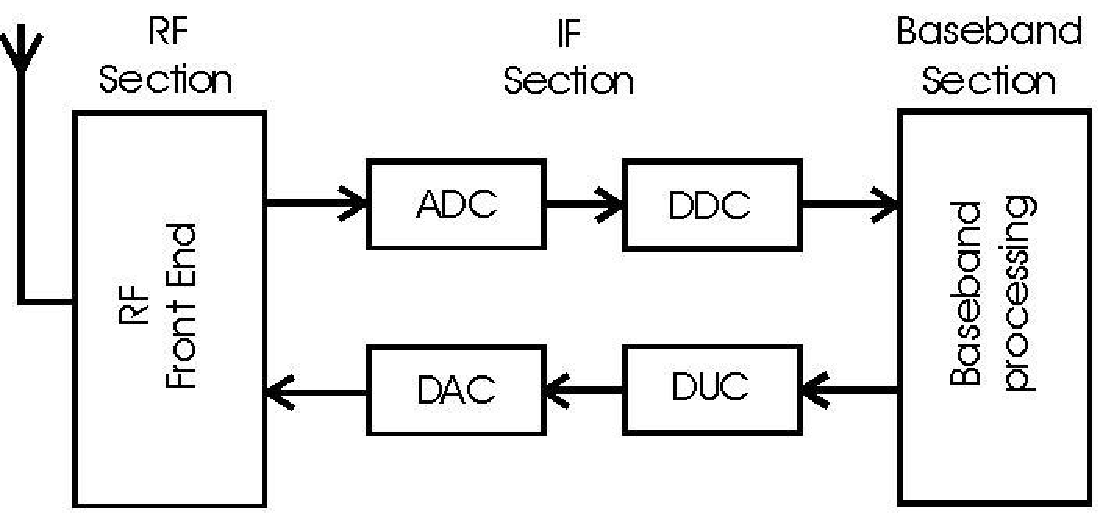
\includegraphics[width=0.7\textwidth]{../images/sdrBlock}
  \caption{Block diagram of SDR.}
  \label{sdrBlock}
\end{figure}

The SDR contains a number of basic functional blocks.
The SDR in general can be divided into three basic sections, namely the front
end, the IF section and the base-band section. The front end section consits 
of analogue RF circuitry that is responsible for the reception and 
transmission of signals at the operating frequency. The IF section performs
the digital to analog conversion and vice versa. It also does various signal 
processing tasks like filtering, modulation and demodulation, digital up 
conversion (DUC), digital down conversion (DDC) etc. The last stage of the 
radio is the baseband processor. It is at this point that the digital data 
gets processed \cite{miller08}\cite{kranthi13}.
We have used GNURadio and USRP N210 to configure the SDR used in implementing
our Cognitive Radio testbed. 

\begin{figure}
  \centering
  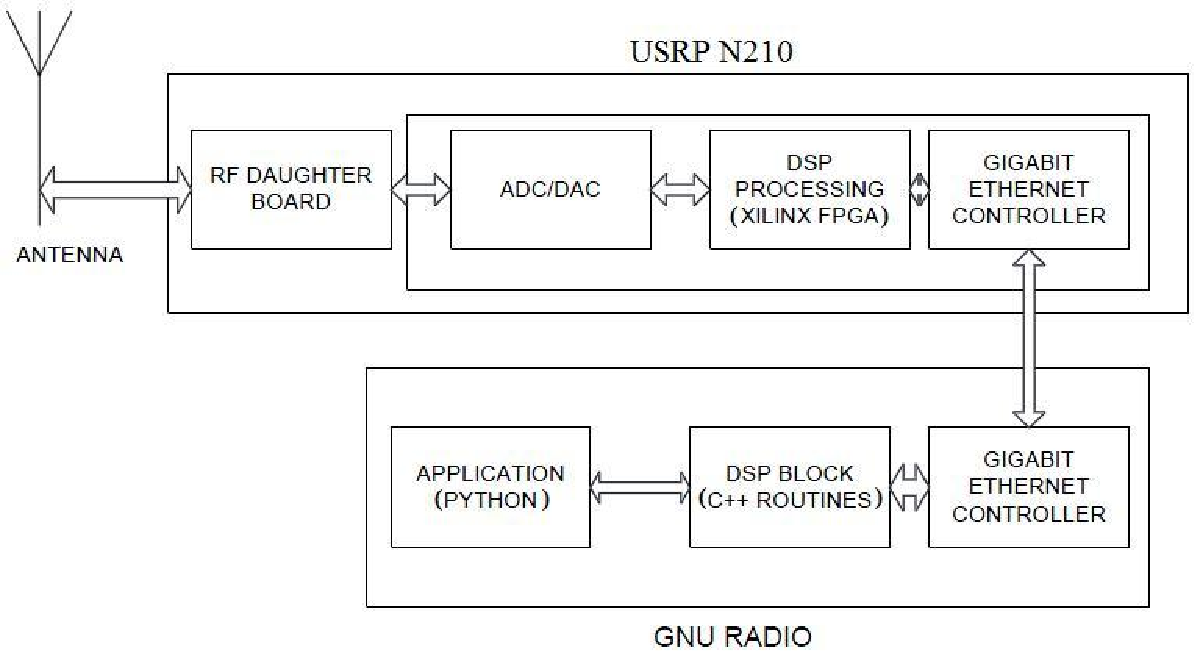
\includegraphics[width=0.7\textwidth]{../images/usrpGNURadioBlock}
  \caption[USRP operation with GNURadio]{Block diagram for the operation of USRP
  with GNURadio.}
  \label{usrpGNURadioBlock}
\end{figure}

A block diagram of a USRP-based SDR transceiver executing a GNURadio based 
application is shown in Figure \ref{usrpGNURadioBlock}. The USRP kit is the 
hardware interface and GNURadio is used for the baseband signal processing
tasks.


\section{USRP}

The USRP (Universal Software Radio Peripheral) is intended to provide a 
low-cost, high quality hardware platform for software radio. It is designed
and marketed by Ettus Research, LLC. It is commonly used by research labs,
universities, and hobbyists. The USRP platform is designed for RF applications
from DC to 6 GHz. USRPs connect to a host computer through a high-speed USB or
Gigabit Ethernet link, which the host-based software uses to control the USRP
hardware and transmit/receive data.

The USRP Hardware Driver (UHD) is the official driver for all Ettus Research
products. The UHD supports Linux, Mac OS X and Windows.

\begin{figure}
\centering
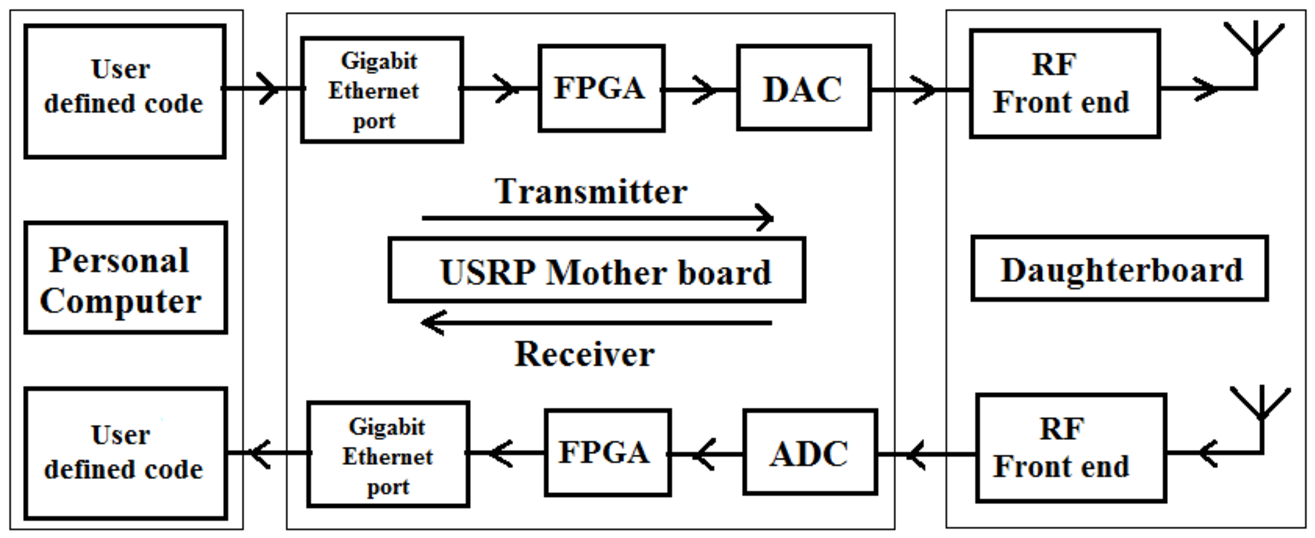
\includegraphics[width=0.9\textwidth]{../images/usrpBlock}
\caption[Block diagram of USRP]{Block diagram of USRP 
\protect\cite{kranthi13}.}
\label{usrpBlock}
\end{figure}

In this project we are using a particular model of USRP product known as the
USRP N210.

\subsection{USRP N210}

The USRP N200 and N210 are the highest performing class of hardware of the 
USRP family of products, which enables engineers to rapidly design and 
implement powerful, flexible software radio systems. The N200 and N210 
hardware is ideally suited for applications requiring high RF performance and
great bandwidth. Such applications include physical layer prototyping, dynamic
spectrum access and cognitive radio, spectrum monitoring, record and playback,
and even networked sensor deployment. The Networked Series products offers 
MIMO capability with high bandwidth and dynamic range. The Gigabit Ethernet
interface serves as the connection between the N200/N210 and the host 
computer. This enables the user to realize 50 MS/s of real-time bandwidth in 
the receive and transmit directions, simultaneously (full duplex).


\section{GNU Radio}

GNU Radio is a free \& open-source software development toolkit that provides 
signal processing blocks to implement software radios. It can be used with 
readily-available low-cost external RF hardware to create software-defined 
radios, or without hardware in a simulation-like environment. It is widely 
used in hobbyist, academic and commercial environments to support both 
wireless communications research and real-world radio systems.

\subsection{What does GNU Radio do?}
It does all the signal processing. You can use it to write applications to 
receive data out of digital streams or to push data into digital streams, 
which is then transmitted using hardware.

GNU Radio has software equivalents of real world radio system components like 
filters, demodulators, equalizers, etc. These are usually referred to as
blocks. You can create a complex system by connecting various blocks. If you
cannot find some specific blocks, you can even create your own blocks and add
them.

Most of GNU Radio has been implemented using the Python programming language,
and the performance-critical parts have been implemented using C++. Typically,
a GNU Radio user writes his applications in Python, unless he has some
performance-critical needs. Thus, GNU Radio gives its users an easy-to-use,
rapid application development environment.

\subsection{GNU Radio with USRP}

\begin{figure}
\centering
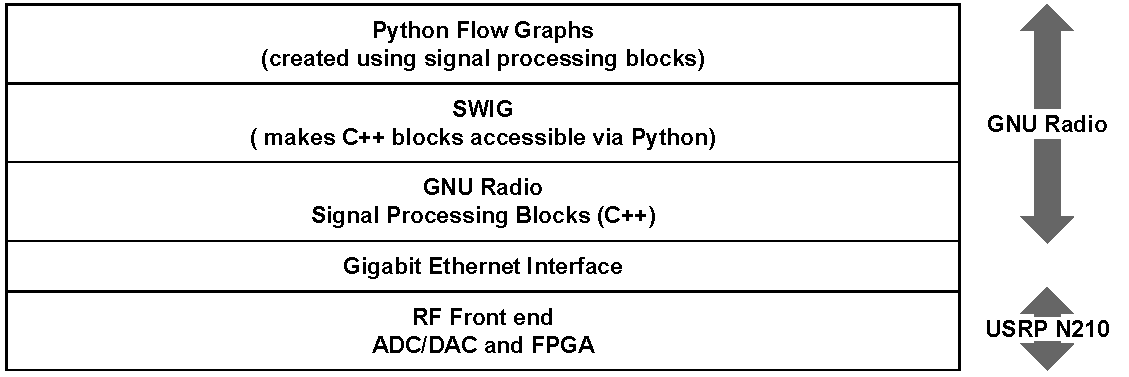
\includegraphics[width=0.9\textwidth]{../images/gnuradio_architecture}
\caption{Architecture of GNU Radio}
\label{gnuradio_architecture}
\end{figure}

The USRP and the host computer make up the hardware part of the SDR system. 
The host computer must run a compatible software package such as GNU Radio or
Simulink to complete the SDR system. In this project we are using GNU Radio
as the software platform.

GNU Radio communicates with the USRP through the USRP Hardware Driver (UHD)
software. The UHD provides a host driver and an Application Programming
Interface (API) for the USRP. GNU Radio uses the UHD to set user-specified
parameters like RF center frequency, antenna selection, gain, sampling rate,
interpolation, decimation, etc.


\chapter{OpenBTS}

OpenBTS is a Unix application that uses a software radio to present a GSM Um interface 
to handsets and uses a SIP softswitch or PBX to connect calls.
The combination of the global-standard GSM air interface with low cost VoIP backhaul 
forms the basis of a new type of cellular network that can be deployed and operated at a much lower
cost than existing technologies in many applications, 
especially rural cellular deployments and private cellular networks in remote areas.

\section{The OpenBTS Application Suite}
A complete OpenBTS installation consists of many distinct applications:

\begin{description}
\item[OpenBTS] The actual OpenBTS application, containing most of the GSM stack above the radio modem.
\item[Transceiver] The software radio modem and hardware control interface.
\item[Smqueue] A store-and-forward server for text messaging.
\item[Asterisk] A VoIP PBX or ``softswitch''.
\item[SIPAuthServe] An application managing the database of subscriber information.
\item[Other Services] Optional services supported through external servers, interfaced to OpenBTS through
various protocol.

\end{description}


\subsection{OpenBTS}
The OpenBTS application contains:
\begin{itemize}
\item L1 TDM functions (GSM 05.02)
\item L1 FEC functions (GSM 05.03)
\item L1 closed loop power and timing controls (GSM 05.08 and 05.10)
\item L2 LAPDm (GSM 04.06)
\item L3 radio resource management functions (GSM 04.08)
\item L3 GSM-SIP gateway for mobility management
\item L3 GSM-SIP gateway for call control
\item L4 GSM-SIP gateway for text messaging
\end{itemize}

The general design approach of OpenBTS is not to implement any function above L3 or L4, so at L3 or L4
every subprotocol of GSM is either terminated locally or translated through a gateway to some other protocol
for handling by an external application. Similarly, OpenBTS itself does not contain any speech transcoding
functions above the L1 FEC parts.


\subsection{Transceiver}
The transceiver application performs the radiomodem functions of GSM 05.05 and manages 
the Gigabit Ethernet interface
(USB2 interface, in case
of USRP1 or older models) to the radio hardware.

\subsection{Smqueue}
Smqueue is an RFC-3428 store-and-forward server that is used for 
text messaging in the OpenBTS system. Smqueue is required to send 
a text message from one MS to another, or to provide reliable 
delivery of text messages to an MS from any source.

\subsection{Asterisk}
OpenBTS uses a SIP router or PBX to perform the 
call control functions that are normally performed by the MSC
in a conventional GSM network, although in 
most network configurations this switching
function is distributed over multiple switches. 
These switches also provide transcoding services.

\subsection{SIPAuthServe}
An application that implements Subscriber Registry, the database of subscriber 
information that replaces both
the Asterisk SIP registry and the GSM Home Location Register (HLR) 
found in a conventional GSM net-
work.




\chapter{Spectrum sensing}

Spectrum sensing is the main task in the entire operation of cognitive
radio. Spectrum sensing is defined as the finding of spectrum holes in 
the local neighborhood of the cognitive radio receiver. Spectrum holes are the
underutilized (in part or in full) subbands of spectrum at a particular time
in a specific location. Moreover for cognitive radio to fulfil its potential
in solving the problem of spectrum underutilization, the spectrum sensing 
method used should be reliable and computationally feasible in real-time 
\cite{haykin09}.

There are many spectrum sensing techniques available. Three important ones of
them are as follows:
\begin{itemize}
    \item Energy detection
    \item Matched filter detection
    \item Cyclostationarity detection
\end{itemize}

\section{Energy detection}

Conventional energy detector is made up of a low pass filter, an A/D 
converter, a square law detector and an integrator (Figure 
\ref{energyDetection}a). This implementation is not flexible enough, 
especially in the case of narrowband signals and sinewaves. Also, this 
requires a pre-filter matched to the bandwidth $B$ of the signal to be scanned
\cite{cabric06}.

So, an alternative implementation is generally used where we find the squared 
magnitude of the FFT using the Average Periodogram method (Figure 
\ref{energyDetection}b). In this architecture, we can alter the bandwidth of
frequencies scanned just by taking
the required number of FFT bins. 

Spectrum sensing can be viewed as a binary hypothesis-testing problem 
\cite{zhang09}:
\begin{itemize}
    \item $H0$: primary user is absent
    \item $H1$: primary user is present
\end{itemize}

The detection is basically to decide between the following two hypotheses,
\begin{align}
    x(t) &= n(t), & H0 \nonumber \\
    x(t) &= h(t)s(t) + n(t), & H1 \nonumber
\end{align}

where $x(t)$ is the received signal, $s(t)$ is the primary user signal, $h(t)$
is the complex channel gain and $n(t)$ is the additive white gaussian noise
(AWGN) with zero mean and variance $\sigma_n^2$. Generally $h(t)$ is assumed
to be constant $h_0$ for the detection period. A statistics $Y$ is computed by
taking energy samples over a time $T$ in a bandwidth $B$ and compared with a 
predefined threshold $\gamma$ for making the decision.

Energy detection is one of the simplest methods of spectrum sensing. It is the 
optimal detection method for unknown signals. Moreover, it is widely used 
because its computationally less resource-intensive.

\begin{figure}
    \centering
    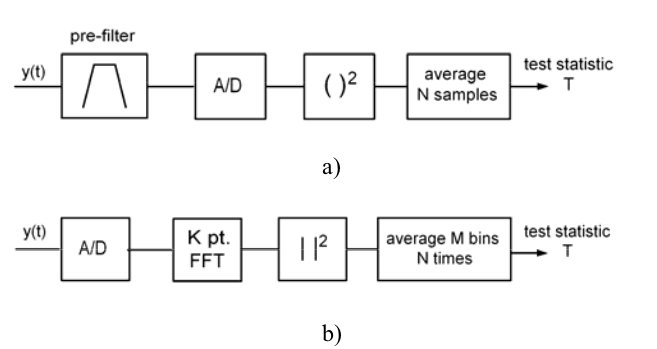
\includegraphics[width=0.7\textwidth]{energyDetection}
    \caption[Energy Detection block diagram]{(a) Implementation using analog 
    filter and square law device \\
    (b) Implementation using periodogram. \\
    \footnotesize{Source: \cite{cabric06}}}
    \label{energyDetection}
\end{figure}

But this method is not without problems. It is always to difficult to 
determine a threshold that will work for all situations. This method cannot
say whether an interfering signal is from a primary user or a secondary user.
Low SNR (signal to noise ratio) signals cannot be detected easily.

The frequency resolution can be improved by increasing N, the number of FFT 
points, but then this requires more samples and thereby takes more time.

\section{Matched filter detection}
A matched filter is a linear filter to maximize the output SNR of a received 
signal. It is the optimum filter to detect signals that are known a priori 
\cite{wikiMF}.

\begin{figure}
\centering
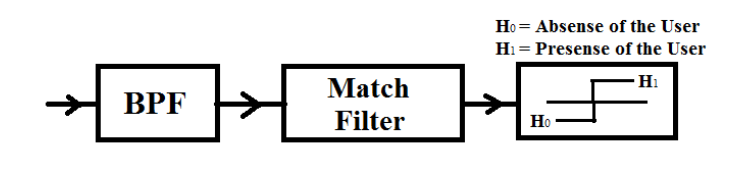
\includegraphics[width=0.8\textwidth]{matchedFilter}
\caption[Matched filter]{Block diagram of Matched filter implementation.}
\label{matchedFilter}
\end{figure}

In matched filtering, the received signal is first band pass filtered and then
convolved with the impulse response. The impulse response $h$ here is the 
reference signal itself \cite{bhatta11}. Matched filtering is so called 
because the impulse response is matched to the reference signal.
\begin{equation*}
    Y[n] = \sum_{-\infty}^{\infty} h[n-k]x[k]
\end{equation*}

Here, $x[k]$ is the received or unknown signal with additive noise.
The goal of matched filtering is to enhance the component of reference signal
in the received signal and to suppress the noise. This works best when the 
additive noise is completely orthogonal to the reference signal or when the
noise is completely Gaussian. In practice though, the noise doesn't turn out 
to be purely Gaussian.
 
Matched filtering requires only $O$(1/SNR) samples to meet a given $P_d$, 
probability of detection requirement. Thus it requires less detection time.

But, matched filtering requires us to have a priori information about the 
received signal. This technique requires demodulating the received signal. For
demodulation, we require information like bandwidth, operating frequency, 
modulation type, pulse shaping, packet format, etc. Demodulating the received
signal correctly also requires timing synchronization, carrier 
synchronization, etc. It might still be possible to achive this because the
received data carry preambles, synchronization data, etc.

This method requires a specific type of receiver for every primary user.
Implementing this method on a receiver will scale up the complexity and the 
power consumption greatly.

\section{Cyclostationarity detection}



\chapter{Implementation of cognitive radio using OpenBTS}

In our project we are able to successfully demonstrate the
coexistence of primary users and secondary users in the same 
frequency channel in the
GSM band. In order to accomplish this, we have implemented
a cognitive radio which detects the spectrum holes in the
radio spectrum and enables secondary users to utilize these 
for communication. An experimental setup has been  
developed for this demonstration using OpenBTS and GNU 
radio software and USRP N210 as hardware.

Experimental setup diagram:


\section{Description of setup}
The figure above describes the experimental setup for a
two-frequency system. The primary system has only
one USRP as an RF front and it runs OpenBTS. The 
secondary system has two USRP kits connected to it and one of them
runs OpenBTS and the other GNURadio.
This secondary system has cognitive capabilities. 
To provide cognitive capabilities it was required that 
OpenBTS and GNU radio run together in the same system and 
talk to each other which was challenging. Secondary system
continuously senses the frequency band of interest and does 
decision making depending upon the analysis of the data 
collected and changes its parameters accordingly so that 
primary and secondary users coexist. The spectrum sensing 
is accomplished by using GNU radio. Also we made GNU radio 
and OpenBTS coordinate to behave in appropriate manner and 
take dynamic decisions as and when required to make over all
system behave in a cognitive manner.

First a two-frequency cognitive system is developed.
For this two GSM bands are used with centre frequency
945 MHz (F1) and 950 MHz (F2). Secondary users are made to occupy
one of these two bands say F1. Then we make the primary users 
enter the same band. This results in an increase in energy 
levels in this band which is sensed by the secondary system 
as it continuously scans this band. Immediately
secondary users are shifted to other frequency band (F2)
there by vacating F1 for primary users. Hence a two-frequency
cognitive system demonstrating coexistence of a pair of
primary and secondary users is accomplished. 

The whole technique is described using a flow graph below:

Flow graph here :

Now this two frequency system is expanded to a 
four frequency system where we have F1 = 936 MHz, 
F2 = 943 MHz, F3 = 950 MHz, F4 = 957 MHz. The experimental setup
is also expanded with two primary systems and one secondary
system. Each primary system has an USRP kit running OpenBTS and
the secondary system has two USRP kits connected to it, one for OpenBTS
and the other one for GNURadio, as we had previously in the two-frequency 
system.
 
Figure for 4 frequency system here:


Here we make a pair of primary users occupy one of the four
frequency channel say F2. We make secondary users use a frequency channel
say F1. Now the other pair of primary users try to enter frequency
F1 for communication. This is sensed by the secondary system 
and it tries to migrate secondary users to F2 which also happens to be 
occupied already. Our secondary system detects that F2 is occupied and
therefore moves on to find a spectrum hole in the four-frequency 
spectrum. It finds that frequency F3 is unoccupied and thus
allows secondary users to enter F3 and utilize it for communication.
The difference between a four-frequency system and a two-frequency system is 
that the secondary system in a four-frequency
system has to first check the presence of primary users before 
switching into a particular frequency channel.
This was not the case in the two-frequency system. In the
two-frequency system we assumed that the other band is always 
unoccupied at the time of switching as only a pair of primary
users existed and thereby only a single band is always unoccupied.


The following flow graph describes the four frequency cognitive system:

Flow graph here

The spectrum sensing is done by energy detection technique and
it was required that a proper threshold be set for decision making. 
A number of readings were taken to decide the noise level, energy 
level when only primary users were active and also energy levels 
when both primary users and secondary users were active in the same band 
for a short duration of time. The threshold value depends on the
power transmitted by the users and their distance from the USRP 
kit which is RF front for GNURadio. This distance dependency can 
be removed by setting the threshold quite lower than required so 
that even if the users move far away the decision making is not
affected. 






\section{CUSUM}
CUMSUM peak detection is also applied after energy detection to ensure that the
detected high energy in the band of interest is not due some  not relevant 
reason like random fluctuations in noise power etc but due to presence of 
primary radio in that band. This ensures high accuracy in primary radio 
detection and correct decision making.
CUSUM is basically a sequential analysis technique to monitor change detection. 
It is a criterion for deciding when to take corrective action. As the name 
implies CUSUM involves calculating cumulative sum. This makes it sequential. 
The samples from process  are assigned weights  and summed as followed,

\begin{align}
S_0 &= 0; \nonumber \\
S_{n+1} &= max(0, S_n + x_n - \omega_n) \nonumber
\end{align}
When the value of  exceeds a certain threshold value a change  in value has 
been found. This formula detects change only in positive direction. To detect 
change in negative direction we have to do min operation instead of max 
operation and the change in value is detected when goes below threshold.







\section{Tasks over the year}
The next section of this chapter gives a step by step description of tasks we 
accomplished during our project tenure. 

\begin{enumerate}

\item We began with exploring with what cognitive radio is and how it can be used 
in the already existing radio. We did literature survey on the ongoing work in 
context to cognitive radio. 
\item We learned GNU Radio software package starting from its installation. We 
also designed FM receiver using GNU Radio Companion to get use to the software. 
Also we tried and learn the codes of already existing signal processing blocks 
that GNU Radio provides.
\item GNU Radio applications are primarily written using the Python programming 
language and hence we learned Python language.
\item USRP N2 kit is used as hardware in our project. We got use to this kit and 
also did range testing of this kit to ensure distance is not a major factor in 
our decision making algorithm and can be neglected.
\item The next task was to understand the working of OpenBTS software. Starting 
from the installation of this software we registered our GSM SIM cards in the 
local network established by OpenBTS. We could perform calling and SMS sending 
between our phones using the local network established by Open BTS with USRP 
kit as hardware end.
\item Since spectrum sensing is major part of cognitive radio literature survey 
on various spectrum sensing techniques was done. We choose energy detection 
spectrum sensing technique for our project and so we did detail study of a 
technique called Average Periodogram Analysis to implement this method. We also 
simulated this technique in Matlab using various windowing methods and 
understand results. 
\item After all this we designed our problem statement and the flow graph of 
how we will approach the problem which we have included in the last chapter. 
Also we decided upon building the experimental setup which we have covered in 
the start of this chapter. 
\item  First key step to approach this problem was to run Open BTS and GNU 
Radio together in the same computer with two USRP kits connected one for Open 
BTS and other for GNU radio. It was a little tricky. \textbf{Why tricky u 
include here regarding the IP conflict an all}
\item The next was to build a two frequency cognitive system with a pair of 
primary and secondary users communicating in parallel and primary pair having 
higher priority when ever both try to use same radio band. Detail description 
of this is in the start of this chapter.
\item This two frequency system was expanded to four frequency system with two 
primary pair of users and one secondary pair of users coexisting. This 
demonstrated that both primary and secondary users can exist in the same GSM 
Network without affecting the existing system.
\end{enumerate}
\chapter{Conclusion and Future Work}

\section{Conclusion}
The rapid growth in the number of cell phones and other wireless devices has 
brought about a scarcity of spectral resources. This is further worsened by the
inefficient usage of the spectrum. Cognitive Radio has a lot of potential to solve this problem
by finding the spectrum holes and enabling secondary users to utilize them. CR 
thereby increases the number of mobile device users possible by putting 
underutilized frequency bands into use. We have 
demonstrated the capabilities of CR by developing a 2-frequency CR Test-Bed and
a 4-frequency CR Test-Bed and successfully testing them out.  We have shown
that the secondary users yield the frequency channel they have been utilizing
for communication as soon as the presence of primary users is detected thus
giving a higher priority to the primary users.


\section{Future work}
To detect the presence of active primary users, we have used energy detection 
based spectrum sensing method to measure the energy level at the uplink 
frequency of the primary BTS. This energy level is dependent
on the distance of the primary users from the sensing unit. Thus, our criteria
for determining the presence of primary users is distance dependent. 
In future, this dependency could be removed by resorting to better 
spectrum sensing techniques.

When our secondary system switches to a new underutilized frequency band, the
secondary calls get dropped and have to be restarted. Better
algorithms could be designed to avoid this call drop from happening.

\appendix
\chapter{Codes}

\section{Code for the two-frequency system}


\subsection{freq2secondaryBTS.py}

This code was written to demonstrate the two-frequency system.
This code was written by modifying the already available program named 
``usrp\_spectrum\_sense.py'' that comes together with the GNURadio software
package. We set the 
default UHD device address to ``192.168.20.2'' because that is the IP address
of the USRP device we are using as a spectrum sensor. The default samping rate
was set to 1e6 i.e. 1MHz. The default FFT size is given as 'sampling rate /
channel bandwidth'. We wanted an FFT size of 1024 so we set the bandwidth to
976.56 Hz since 1 MHz / 976.56 Hz $\approx$ 1024.

The class 'my\_top\_block' was modified by replacing the lines:
\begin{lstlisting}[language=Python]

        self.channel_bandwidth = options.channel_bandwidth

        self.min_freq = eng_notation.str_to_num(args[0])
        self.max_freq = eng_notation.str_to_num(args[1])

        if self.min_freq > self.max_freq:
            # swap them
            self.min_freq, self.max_freq = self.max_freq, self.min_freq    
\end{lstlisting}
with the lines
\begin{lstlisting}[language=Python]
        self.channel_bandwidth = options.channel_bandwidth

        self.down_freq = eng_notation.str_to_num(args[0])
        self.up_freq = (self.down_freq) - 45e6    
\end{lstlisting}

The method 'set\_next\_freq' of the class 'my\_top\_block' was modified by
replacing
\begin{lstlisting}[language=Python]
        target_freq = self.next_freq
        self.next_freq = self.next_freq + self.freq_step
        if self.next_freq >= self.max_center_freq:
            self.next_freq = self.min_center_freq
\end{lstlisting}
with
\begin{lstlisting}[language=Python]
        target_freq = self.up_freq
\end{lstlisting}




In the code listing that follows we have listed only the functions that we
customized and the ones that we added.

\begin{lstlisting}[language=Python]
def main_loop(tb):
    startOpenBTS(tb.down_freq,tb)

    
def sub_loop(tb):

    # use a counter to make sure power is less than threshold
    # lowPowerCount = 0
    # lowPowerCountMax = 10
    print 'fft size', tb.fft_size
    N = tb.fft_size
    mid = N // 2
    cusum = 0
    counter = 0
    

    while 1:

        # Get the next message sent from the C++ code (blocking call).
        # It contains the center frequency and the mag squared of the fft
        m = parse_msg(tb.msgq.delete_head())

        # m.center_freq is the center frequency at the time of capture
        # m.data are the mag_squared of the fft output
        # m.raw_data is a string that contains the binary floats.
        # You could write this as binary to a file.



        center_freq = m.center_freq
        bins = 102
        power_data = 0
        noise_floor_db = 0 ## 10*math.log10(min(m.data)/tb.usrp_rate)
        
        for i in range(1, bins+1):
            power_data += m.data[mid-i] + m.data[mid+i]
        power_data += m.data[mid]
        power_data /= ((2*bins) + 1)
        
        power_db = 10*math.log10(power_data/tb.usrp_rate) - noise_floor_db
        power_threshold = -59.0
        
        

        #if (power_db > tb.squelch_threshold) and (power_db > power_threshold):
            #print datetime.now(), "center_freq", center_freq, "power_db", power_db, "in use"
            # lowPowerCount = 0
        #else:
        print datetime.now(), "center_freq", center_freq, "power_db", power_db
            # lowPowerCount += 1

        # if (lowPowerCount > lowPowerCountMax):
        # down_freq = center_freq + 45e6
        # startOpenBTS(down_freq)
        # break

        #cusum cusum cusum is here
        cusum = max(0, cusum + power_db - power_threshold)
        if (cusum > 0):
            counter += 1
            if (counter > 2):
                print "CUSUM is now positive!!!"
                down_freq = center_freq + 45e6
                quitOpenBTS(down_freq, tb)
                break

                
def startOpenBTS(downFrequency,tb):
    
    
    arfcn=int((downFrequency-935e6)/2e5)
    if (arfcn < 0):
        print "ARFCN must be > 0 !!!"
        sys.exit(1)
    print 'ARFCN=', arfcn
    #DB modifications
    t=(arfcn,)
    conn=sqlite3.connect("/etc/OpenBTS/OpenBTS.db")
    cursor=conn.cursor()
    cursor.execute("update config set valuestring=? where keystring='GSM.Radio.C0'",t)
    conn.commit()

    #start the OpenBTS
    f=subprocess.Popen(os.path.expanduser('~/ddpOpenBTS/runOpenBTS.sh'))
    f.wait()
    tb.msgq.delete_head()
    time.sleep(0.25)
    sub_loop(tb)


def quitOpenBTS(downFreq, tb):
    f=subprocess.Popen(os.path.expanduser('~/ddpOpenBTS/quitOpenBTS.sh'))
    f.wait()
    if downFreq <= 945e6:
        newDownFreq = downFreq + 10e6
    else:
        newDownFreq = downFreq - 10e6

    tb.up_freq = newDownFreq - 45e6
    print "new tb.up_freq: ", tb.up_freq
    startOpenBTS(newDownFreq, tb)
\end{lstlisting}






\section{Code for the four-frequency system}
\subsection{secondaryBTS.py}

Most of the code is similar to ``freq2secondaryBTS.py''. The only modified 
functions are listed below:

\begin{lstlisting}[language=Python]

def main_loop(tb):
    startOpenBTS(tb.down_freq,tb)


def sub_loop(tb):

    print 'fft size', tb.fft_size
    N = tb.fft_size
    mid = N // 2
    cusum = 0
    counter = 0
    

    while 1:

        # Get the next message sent from the C++ code (blocking call).
        # It contains the center frequency and the mag squared of the fft
        m = parse_msg(tb.msgq.delete_head())

        # m.center_freq is the center frequency at the time of capture
        # m.data are the mag_squared of the fft output
        # m.raw_data is a string that contains the binary floats.
        # You could write this as binary to a file.



        center_freq = m.center_freq
        bins = 102
        power_data = 0
        noise_floor_db = 0      ##  10*math.log10(min(m.data)/tb.usrp_rate)
        
        for i in range(1, bins+1):
            power_data += m.data[mid-i] + m.data[mid+i]
        power_data += m.data[mid]
        power_data /= ((2*bins) + 1)
        
        power_db = 10*math.log10(power_data/tb.usrp_rate) - noise_floor_db
        power_threshold = -70.0
        
        print datetime.now(), "center_freq", center_freq, "power_db", power_db

        #cusum cusum cusum is here
        cusum = max(0, cusum + power_db - power_threshold)
        if (cusum > 0):
            counter += 1
            if (counter > 2):
                print "CUSUM is now positive!!!"
                down_freq = center_freq + 45e6
                quitOpenBTS(down_freq, tb)
                break
        else:
            counter = 0




def startOpenBTS(downFrequency,tb):
    arfcn=int((downFrequency-935e6)/2e5)
    if (arfcn < 0):
        print "ARFCN must be > 0 !!!"
        sys.exit(1)
    print 'ARFCN=', arfcn
    #DB modifications
    t=(arfcn,)
    conn=sqlite3.connect("/etc/OpenBTS/OpenBTS.db")
    cursor=conn.cursor()
    cursor.execute("update config set valuestring=? where keystring='GSM.Radio.C0'",t)
    conn.commit()

    #start the OpenBTS
    f=subprocess.Popen(os.path.expanduser('~/ddpOpenBTS/runOpenBTS.sh'))
    f.wait()
    tb.msgq.delete_head()
    time.sleep(0.25)
    sub_loop(tb)
              

def quitOpenBTS(downFreq, tb):
    f=subprocess.Popen(os.path.expanduser('~/ddpOpenBTS/quitOpenBTS.sh'))
    f.wait()    
    newDownFreq = getNewChannel(downFreq, tb)
    startOpenBTS(newDownFreq, tb)

        

def getNewChannel(downFreq, tb):
    newDownFreq = downFreq + 7e6
    if newDownFreq > 960e6:
        newDownFreq = 936e6

    tb.up_freq = newDownFreq - 45e6
    print "new tb.up_freq: ", tb.up_freq
    tb.msgq.delete_head()
    time.sleep(0.25)

    print 'fft size', tb.fft_size
    N = tb.fft_size
    mid = N // 2
    cusum = 0
    counter = 0
    loopcounter = 0
    

    while loopcounter < 10:

        # Get the next message sent from the C++ code (blocking call).
        # It contains the center frequency and the mag squared of the fft
        m = parse_msg(tb.msgq.delete_head())


        center_freq = m.center_freq
        bins = 102
        power_data = 0

        
        for i in range(1, bins+1):
            power_data += m.data[mid-i] + m.data[mid+i]
        power_data += m.data[mid]
        power_data /= ((2*bins) + 1)
        
        power_db = 10*math.log10(power_data/tb.usrp_rate)
        power_threshold = -70.0
        
        
        print datetime.now(), "center_freq", center_freq, "power_db", power_db
        print "precheck"

        #cusum cusum cusum is here
        cusum = max(0, cusum + power_db - power_threshold)
        loopcounter += 1
        if (cusum > 0):
            counter += 1
            if (counter > 2):
                print "CUSUM is now positive!!!"
                newDownFreq = getNewChannel(newDownFreq, tb)
                break
        else:
            counter = 0
    return newDownFreq

\end{lstlisting}




\section{primaryBTS.py}
\begin{lstlisting}[language=Python]
#!/usr/bin/env python


import sys
import sqlite3
import os
import re

def main_loop():
    usage = "usage: %prog channel_freq"
    if len(sys.argv) != 2:
        print 'usage:', sys.argv[0], 'channel_freq'
        sys.exit(1)


    center_freq = int(re.match(r'\d+', sys.argv[1]).group())*1e6
    startOpenBTS(center_freq)

def startOpenBTS(frequency):            
    
    arfcn=int((frequency-935e6)/2e5)
    print 'ARFCN=', arfcn
    
    #DB modifications
    t=(arfcn,)
    conn=sqlite3.connect("/etc/OpenBTS/OpenBTS.db")
    cursor=conn.cursor()
    cursor.execute("update config set valuestring=? where keystring='GSM.Radio.C0'",t)
    conn.commit()
    
    #start the OpenBTS
    f=os.popen('~/ddpOpenBTS/runOpenBTS.sh')
    f.close()
              

if __name__ == '__main__':

    try:
        main_loop()

    except KeyboardInterrupt:
        pass

\end{lstlisting}


\section{runOpenBTS.sh}
\begin{lstlisting}[language=bash]
#!/bin/bash

sudo echo "Hi, this script starts OpenBTS in Ubuntu 12.04!"
sudo service asterisk restart
sudo gnome-terminal -x sh -c "sudo asterisk -r" &

#cd ~/OpenBTS/
#sudo gnome-terminal --tab -e "sudo smqueue/trunk/smqueue/smqueue" \
#   --tab -e "sudo subscriberRegistry/trunk/sipauthserve" &

cd ~/OpenBTS/openbts/trunk/apps/
sudo gnome-terminal --tab -e "sudo ../../../smqueue/trunk/smqueue/smqueue" \
    --tab -e "sudo ../../../subscriberRegistry/trunk/sipauthserve" &

#sudo gnome-terminal -x sh -c "sudo ./OpenBTS" &
#sudo gnome-terminal -x sh -c "sudo ./OpenBTSCLI" &
sudo gnome-terminal --tab -e "sudo ./OpenBTS" \
    --tab -e "sudo ./OpenBTSCLI" &
cd ~

\end{lstlisting}


\section{quitOpenBTS.sh}
\begin{lstlisting}[language=bash]
#!/bin/bash

sudo echo "Hi, this script turns OpenBTS off in Ubuntu 12.04!"

sudo killall transceiver smqueue sipauthserve OpenBTSCLI asterisk
\end{lstlisting}





\chapter{Installation procedures}
The installation procedures given in this chapter are for the Ubuntu 12.04 LTS
desktop operating system only. For other operating systems, please use the 
internet.
\section{UHD}
\begin{lstlisting}[language=bash]
# Install the runtime dependencies:

sudo apt-get install python libboost-all-dev libusb-1.0-0-dev python-cheetah \
doxygen python-docutils git cmake

# Go to your home folder and git clone the UHD repository:

cd ~
git clone https://github.com/EttusResearch/uhd.git

# Generate Makefiles with CMake:

cd uhd/host
mkdir build
cd build
cmake ../

# Build and install:

make
make test
sudo make install
sudo ldconfig
\end{lstlisting}


\section{OpenBTS}

\begin{lstlisting}[language=bash]
cd ~
mkdir OpenBTS
svn co http://wush.net/svn/range/software/public OpenBTS/

sudo apt-get install autoconf libtool libosip2-dev libortp-dev \
libusb-1.0-0-dev g++ sqlite3 libsqlite3-dev erlang libreadline6-dev \
libncurses5-dev

cd OpenBTS
cd a53/trunk
sudo make install


## for USRP N210 only
cd openbts/trunk
autoreconf -i
./configure --with-uhd
make

#(from OpenBTS root)
cd apps
ln -s ../Transceiver52M/transceiver .

## for USRP N210 only

sudo mkdir /etc/OpenBTS
sudo sqlite3 -init ./apps/OpenBTS.example.sql /etc/OpenBTS/OpenBTS.db ".quit"
sudo sqlite3 /etc/OpenBTS/OpenBTS.db .dump

\end{lstlisting}










\backmatter
\bibliographystyle{plain}
\bibliography{ddpThesis}

\end{document}
